\documentclass{article}

\usepackage{caption}
\usepackage{graphicx, subfig}

\title{\LaTeX \ Notes}
\author{Xmp}
\date{\today}

\begin{document}
\maketitle

%生成目录,初次使用目录,或章节图表等层次结构发生变化时,都需要执行两%遍编译命令才能获得正确结果
\setcounter{tocdepth}{2}%设定目录深度
\tableofcontents %列出目录
\listoffigures %插图目录
\listoftables %表格目录

\begin{abstract}%article和report可以有摘要,book里面没有
	The .tex file is for learing some basic concept.
\end{abstract}

%层次结构,article中没有chapter,而report和book则支持所有层次
\part{part}%Level -1
part 1

%\chapter{chapter}%Level 0
\section{section}%Level 1
section 1

\subsection{subsection}%Level 2
subsection 1

\subsubsection{subsubsection}%Level 3
subsubsection 1

\paragraph{paragraph}%Level 4
paragraph 1

\subparagraph{subparagraph}%Level 5
subparagraph 1


%不想让某些层次的标题出现在目录里
%\chapter*{...}
\section*{don't want to show in the content}
\subsection*{don't want to show in the content}
\subsubsection*{don't want to show in the content}


%字符输入
\# 
\$ 
\~ 
\& 
\_ 
\{ 
\} 
\- 
\textbackslash 
\%

\.{A} \"{A} \={A}  and many other characters.\\

%划线和减号
computer-aided\\
1840--2010\\
to be---or not to be\\
$1-1=0$

%字体样式
\textrm{roman} \\
\textbf{bold face} \\
\textsf{sans serif} \\
\textmd{medium weight} \\
\texttt{typewriter} \\
\textit{italic} \\
\textsc{Samall Caps} \\
\textsl{slanied}\\

%字体相对尺寸
\tiny{sample}\\
\scriptsize{sample}\\
\footnotesize{sample}\\
\small{sample}\\
\normalsize{sample}\\
\large{sample}\\
\Large{sample}\\
\LARGE{sample}\\
\huge{sample}\\
\Huge{sample}\\

%字体强调和下划线,使用ulem宏包可以使用更多的样式
\normalsize
\emph{emphasis}\\
\underline{underline}\\

%换行、换页和断字
%Latex会自动换行或者使用 \\或\newline命令, \newpage强制换页
%自动断字,或者显式指明断字位置
\hyphenation{BASIC blar-blar-blar}
HEllo world HEllo world HEllo world  hello wrodl hello BASIC blar-blar-blar

%长度

%段落对齐,缺省为两端对齐(fully justified)
%\raggedbottom \raggedcenter \raggedleft \raggedright与下面三个环节有相同的功能。
\begin{flushleft}left\\paragraph\end{flushleft} %居左段落
\begin{flushright}right\\paragraph\end{flushright} %居右段落
\begin{center}center\\paragraph\end{center} %段落居中


%缩进和段间距
%LATEX正文中第一个段落缺省不缩进首行,我们可以用identfirst宏包使得第一段也缩进首行。段落首行缩进的距离可以用{\parindent变量来控制,段落之间的距离可以用\parskip变量来控制。
%\usepackage{identfirst}
%\setlength{\parindent}{2em}
%\addtolength{\parskip}{3pt}

%行间距,缺省单倍行距
\begin{figure}
	\centering
	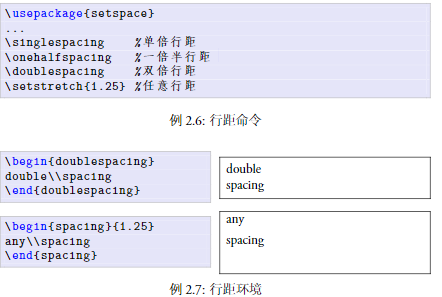
\includegraphics[width=1.0\textwidth]{linespace.png} %linespace.png是图片文件的相对路径
	\caption{linespace} %caption是图片的标题
	\label{img} %此处的label相当于一个图片的专属标志,目的是方便上下文的引用
\end{figure}


\end{document}